% CHAPTER 2

\chapter{Design of a digital ARTVA \label{ch:chapter2}}
\minitoc
%% Enlarge array size
\renewcommand{\arraystretch}{2}

In this chapter we will try to design a digital receiver for the ARTVA signal. Before starting with the design, \emph{ARTVA signal} is deeply analyzed, with the derivation of a simplified model for a field pattern that could be used  for the implementation of the searching algorithm. After that, ferrite antennas are studied, as they are the only way to receive such a long wavelength. In the last part of the chapter the circuitry for the ARTVA receiver is shown and explained.

\section{Analysis of transmitting pattern}

A formal model of the transmitting pattern is fundamental for the implementation of the searching algorithm. We start from the basic Maxwell's equation and we arrive to a simpler model numerically usable.

As we will see, radiating pattern is quite complex due to the fact that we are working in the \textbf{near--field} region, condition that constraint us to not use classical DoA\marginnote{\emph{DoA}: Direction of Arrival}, such as MUSIC or ESPRIT, that operates in far-field condition and at higher frequencies. DoA systems for long waves usually requires too big electro--mechanical devices.

\subsection{Maxwell's Equations}
The following investigation is based upon Maxwell's Equation, in which the magnetic permeability $\magperm$ and dielectric constant $\dielettrico$ are considered constant (the radiation is assumed to propagate at speed of light in air). Also we consider some field properties, that are function of radio distance $\radiodist$ and time $t$:
\[
f(\radiodist,t) = f \qquad f \in \left[\; \chargedens,\; \currdens,\; \efield,\; \bfield,\; \hfield \; \right]
\]
The equations that rule the induction are the \emph{Gauss equation of magnetic induction} and the \emph{Faraday law of electric induction}:
\begin{equation}
\nabla\cdot\bfield = 0
\label{eq:gauss1}
\end{equation}
\begin{equation}
\nabla\times\efield = -\partialt \bfield
\label{eq:faraday}
\end{equation}
while the equations that rule the interaction with materials are \emph{Gauss equation} and \emph{Ampere law}:
\begin{equation}
\nabla\cdot\efield = \dfrac{\chargedens}{{\dielettrico}_0}
\label{eq:gauss2}
\end{equation}
\begin{equation}
\nabla\times\bfield = {\magperm}_0 \left( \currdens + {\dielettrico}_0 \partialt \efield \right)
\label{eq:ampere}
\end{equation}

\subsection{EM field dynamic potentials}

Starting from equation \ref{eq:gauss1}, we can define a vectorial function called \emph{potential vector} $\afield$ of $\bfield$:
\begin{equation}
\bfield = \nabla\times\afield
\label{eq:potvett}
\end{equation}
\marginnote{The existence of $\afield$ is verified by property of $\nabla$ operator, whom states that the divergence of a curl of a vector field is zero\citep{bramanti2009analisi}} 
We insert \ref{eq:potvett} in \ref{eq:faraday}:
\[
\nabla\times\efield = - \partialt \left( \nabla\times\afield \right)
\]
\begin{equation}
\nabla\times\left( \efield + \partialtarg{\afield} \right) = 0
\end{equation}
From the previous equation it is evident that the argument between parentheses is an irrotational vector field, thus a potential function exists such that:
\[
-\nabla\scpot = \efield + \partialtarg{\afield}
\]
and we derive the following definition of electric field:
\begin{equation}
\efield = - \nabla \scpot - \partialtarg{\afield}
\label{eq:efieldvett}
\end{equation}
Equation \ref{eq:potvett} and \ref{eq:efieldvett} are used to express a new formulation for the Maxwell's equation based upon vector potential\sidenote{The proof is in chapter appendix \ref{eq:evidence1}}:
\begin{equation}
\begin{array}{rcl}
\nabla^2\scpot + \partialt \nabla \cdot \afield & = & - \dfrac{\chargedens}{\dielettrico_0} \\
\nabla^2 \afield - \dfrac{1}{\velocitaluce^2} \partialttarg{\afield} - \nabla\left( \nabla \cdot \afield + \dfrac{1}{\velocitaluce^2} \partialtarg{\scpot} \right) & = & -\magperm_0 \currdens
\end{array}
\label{eq:potvecmaxwell}
\end{equation}
Those equation, even if complex, could be resolved with a well posed boundaries condition problem. Equation are coupled with the current formulation, but could be decoupled using the \textbf{Gauge transformation}\citep{mencuccini1988fisica}, also called \textbf{recalibration map}, that is in the form:
\begin{equation}
\left\{ \begin{array}{rcl}
\afield' & \mapsto & \afield + \nabla \lorentz \\
\scpot' & \mapsto & \scpot - \partialtarg{\lorentz}
\end{array}
\right.
\end{equation}
in which $\lorentz = \lorentz(\radiodist,t) \in C^2$. As proofed in \ref{eq:prooftransformationmap}, this map represents an invariant with respect to dynamic potential formulation. If we consider a $\lorentz$ such that it verifies the \textbf{Lorentz equation}
\begin{equation}
\nabla \cdot \afield' = - \dfrac{1}{\velocitaluce^2} \partialtarg{\scpot'}
\end{equation}
we obtain the decoupled version:
\begin{equation}
\begin{array}{rcl}
\nabla^2 \scpot - \dfrac{1}{\velocitaluce^2} \partialttarg{\scpot} & = & - \dfrac{\chargedens}{\dielettrico_0} \\
\nabla^2 \afield - \dfrac{1}{\velocitaluce^2} \partialttarg{\afield} & = & - \magperm_0 \currdens 
\end{array}
\end{equation}
Those dynamic equations describe the time evolution of an EM--field. If field sources are located in a finite region, the problem admit as solution a generalization of the well know stationary formulation, called retarded potential:
\begin{equation}
\begin{array}{rcl}
\scpot(\radiodist,t) & = & \dfrac{1}{4\pi \dielettrico_0} \displaystyle\iiint\limits_{\Omega} \dfrac{1}{\mid \radiodist - \radiodist' \mid} \chargedens\left( \radiodist',t-\dfrac{\mid \radiodist - \radiodist' \mid}{\velocitaluce} \right) d\radiodist   \\
\afield(\radiodist,t) & = & \dfrac{\magperm_0}{4\pi} \displaystyle\iiint\limits_{\Omega} \dfrac{1}{\mid \radiodist - \radiodist' \mid} \currdens\left( \radiodist',t-\dfrac{\mid \radiodist - \radiodist' \mid}{\velocitaluce} \right) d\radiodist 
\end{array}
\end{equation}
in which the vector distance ${\radiodist - \radiodist'}$ is the distance between the point where retarded potential is evaluated and the point where the element of volume $d\radiodist$ of the localized sources is located. The delay is due to the definition of time:
\[
t_r = t - \dfrac{\mid \radiodist - \radiodist' \mid}{c}
\]

\subsection{Magnetic dipole radiation}

\myparagraph{Potential of a magnetic dipole}
Our antenna may be seen as an ideal magnetic dipole\citep{balanis2012antenna}. The transmitting antenna is a solenoid with a ferrite core, that acts as source of the electro--magnetic field. The source is subject to a dipole magnetic moment induced by the current $J = J_0 \cos(\omegaarva t)$, with no free charges (null scalar potential). 
\begin{figure}[h]
	\centering
	
	\tdplotsetmaincoords{60}{130}
	\begin{tikzpicture}[auto,>=latex,tdplot_main_coords]
		\coordinate (origin) at (0,0,0);
		
		% Axis
		\draw [->] (origin) -- (4,0,0) node[anchor=north east]{\scriptsize{$x$}}; \draw (origin) -- (-0.2,0,0);
		\draw [->] (origin) -- (0,4,0) node[anchor=north west]{\scriptsize{$y$}}; \draw (origin) -- (0,-0.2,0);
		\draw [->] (origin) -- (0,0,2) node[anchor=south]{\scriptsize{$z$}}; \draw (origin) -- (0,0,-0.2);

		\tdplotdrawarc[->,line width=3]{(0,0,0)}{2.7}{90}{360+80}{}{}
		\tdplotdrawarc[line width=6]{(0,0,0)}{2.7}{25}{35}{}{}
		\tdplotdrawarc[<->]{(0,0,0)}{3.5}{0}{30}{anchor=north west,xshift=-10}{$\varphi'$}
		\coordinate (drpoint) at (30:2.7);
		\node at (-2.3,2.3,0) {$\mathbf{J}$};
		\node [at=(drpoint),xshift=5,yshift=-10] {$d\mathbf{r}$};

		\node [circle,draw,inner sep=1pt, fill=black] at (7.5,0,6) (rpoint) {};
		\draw[->] (origin) -- node[pos=0.8,above]{$\mathbf{r}$} (rpoint);
		\draw [dashed] (rpoint) -- (7.5,0,0) -- ++(-2.5,0,0);
		\coordinate [at=(drpoint),yshift=3] (drpoint2);
		\draw [<->] (rpoint) -- node[pos=0.425,below,xshift=-22]{$\kappa=|\mathbf{r}-\mathbf{r}'|$} (drpoint2);
		\draw [->] (origin) -- node[right]{$\mathbf{r}'$} (drpoint2);

		\tdplotsetrotatedcoords{90}{90}{180}
		\tdplotsetrotatedcoordsorigin{(origin)}
		\draw[tdplot_rotated_coords,<->] (0.5,0) arc (0:52.5:0.5) node[left,xshift=5,yshift=10]{$\theta$};

		\tdplotsetrotatedcoords{29.5+270}{-23.75}{0}
		\tdplotsetrotatedcoordsorigin{(origin)}
		\draw[tdplot_rotated_coords,<->] (0.75,0) arc (0:90:0.75) node[left,xshift=-15,yshift=10]{$\psi$};
		
	\end{tikzpicture}
	\tdplotsetmaincoords{0}{0}

	\caption{Formulation of magnetic dipole problem}
	\label{eq:dipolomagnetico}
	\forceversofloat
\end{figure}
The magnetic dipole moment is:
\begin{equation}
\magdipole = \pi r'^2\; J \vrz = m_0 \cos(\omegaarva t) \vrz
\label{eq:dipolodacorrente}
\end{equation}
From figure \ref{eq:dipolomagnetico} we define the retarded potential equation, with ${\kappa = \mid \radiodist-\radiodist'\mid}$:
\[
\afield(\radiodist,t) = \dfrac{\magperm_0}{4\pi}\int{\dfrac{J_0\cos(\omegaarva (t - \kappa/c))}{r}\ccos{\varphi'}d\varphi'}\hat{\boldsymbol{\phi}}
\]
In the hypothesis of ${\radiodist\parallel\vrz\times\vrx}$, we obtain a vector $\afield$ directed along $\vry$:
\[\begin{array}{rcl}
\radiodist & = & r \sin(\theta) \vrx + r \cos(\theta) \vrz \\
\radiodist' & = & r' \cos(\varphi') \vrx + r' \sin(\varphi') \vry \\
\kappa & = & \sqrt{(\radiodist - \radiodist')\cdot(\radiodist - \radiodist')}
\end{array}\]
Those elements in retarded potential formulation lead us to the integral formulation that has only one angular dependency:
\begin{equation}
\label{eq:integraledacalc}
\afield(\radiodist,t) = \dfrac{\magperm_0 J_0 r'}{4\pi}\int\limits_{0}^{2\pi}{\dfrac{\cos(\omegaarva (t - \kappa/c))}{\kappa} \cos(\varphi') d\varphi' \hat{\boldsymbol{\phi}}}
\end{equation}
The solution of this integral is reported in appendix; we recall only the simplification used:
\begin{itemize}
\item we assume $r' \ll r$
\item we assume $r' \ll \lambda = 2\pi c/\omegaarva$
\end{itemize}
that brings us to the following solution:
\begin{equation}
\label{eq:soluzioneint}
\afield(\radiodist,t) = \dfrac{\magperm_0 m_0}{4\pi r}\,\sin(\theta)\left( \dfrac{1}{r} \sin\left(\omegaarva(t-r/c)\right) - \dfrac{\omegaarva}{r}\cos\left(\omegaarva(t-r/c)\right)\right)\hat{\boldsymbol{\phi}}
\end{equation}
in which $m_0$ identifies the total dipole moment, considering also the number of the coils of antenna. The rest of the equation describes the propagation of the transmission in near--field conditions.

\myparagraph{Electric and magnetic field}
With null scalar potential we obtain the electric field and the magnetic field from the equations:
\begin{equation}
\begin{array}{rcl}
\efield & = & - \partialtarg{\afield} \\
\bfield & = & \nabla\times\afield 
\end{array}
\end{equation}
The application of differential operator $\nabla$:
\marginnote{In polar coordinates: \newline $\nabla=\left[ \begin{array}{c} \dfrac{\partial}{\partial r} \\ \dfrac{1}{r}\;\dfrac{\partial}{\partial\theta} \\ \dfrac{1}{r \sin(\theta)}\;\dfrac{\partial}{\partial\phi} \end{array} \right]$}
\begin{equation}
\efield = \left[ \begin{array}{c} 0 \\ 0 \\ \partialtarg{A_{\phi}} \end{array} \right]
\qquad
\bfield = \left[ \begin{array}{c} \dfrac{1}{r}\;\dfrac{\partial A_{\phi}}{\partial \theta} \\ - \dfrac{\partial A_{\phi}}{\partial r} \\ 0 \end{array} \right]
\end{equation}
The final formulation for th EM field of a magnetic dipole is\citep{knoepfel2008magnetic}:
\begin{equation}
\begin{array}{rcl}
\label{eq:campidef1}
\tau & = &  t - \dfrac{r}{\velocitaluce} \\
E_{\phi} & = & \dfrac{\magperm_0 m_0}{4\pi}\sin(\theta)\left( \dfrac{\omegaarva}{r^2}\sin\left( \omegaarva\tau \right) + \dfrac{\omegaarva^2}{c}\cos\left( \omegaarva\tau \right) \right) \\
B_{r} & = & \dfrac{\magperm_0 m_0}{2\pi r^2}\cos(\theta)\left( \dfrac{1}{r}\cos\left( \omegaarva\tau \right) + \dfrac{\omegaarva}{c}\sin\left( \omegaarva\tau \right) \right) \\
B_{\theta} & = & \dfrac{\magperm_0 m_0}{4 \pi r^3 c^2}\sin(\theta)\left( \left( \velocitaluce^2 - \omegaarva^2 r^2 \right)\cos\left( \omegaarva\tau \right) + \omegaarva r \velocitaluce \sin\left( \omegaarva\tau \right) \right) 
\end{array}
\end{equation}
In figure \ref{fig:animazionifield} are shown some animation referred to the magnetic field defined in the previous equations. The animation are performed using ARTVA typical parameters, even if time is scaled. The equations are parametric with respect to a value, $m_0$ that is the transmitter magnetic dipole. As we have seen in chapter \ref{ch:chapter1}, the real transmitting power of an avalanche beacon is not known, but it shall have the maximum at \num{10}\si{\meter} inside a range. The animations consider an unitary magnetic dipole moment.

\begin{figure*}[p]
\label{fig:animazionifield}
\animategraphics[width=6.5cm,autoplay,loop]{15}{ch2/img/xz_10m/animation_}{0}{59}
\animategraphics[width=6.5cm,autoplay,loop]{15}{ch2/img/xz_40m/animation_}{0}{59} \newline
\animategraphics[width=6.5cm,autoplay,loop]{15}{ch2/img/xz_100m/animation_}{0}{59}
\animategraphics[width=6.5cm,autoplay,loop]{15}{ch2/img/xz_2lambda/animation_}{0}{59} \newline
\animategraphics[width=6.5cm,autoplay,loop]{15}{ch2/img/xy_10m/animation_}{0}{59} 
\animategraphics[width=6.5cm,autoplay,loop]{15}{ch2/img/xy_2lambda/animation_}{0}{59}
\caption{Graphical animation of the magnetic field $\bfield$ with retarded potential formulation. Those graph derives directly from the equations \ref{eq:campidef1}. To see the animations, please use \texttt{Adobe Acrobat viewer}}
\end{figure*}

\subsection{Magnetic field model simplification}
From animations it is evident that the effect of retarded propagation is almost null inside a radius of \num{40}\si{\meter} from the transmitting source, that is roughly the maximum distance at which an avalanche beacon receives the signal. This brings us to other simplifications for our model, as we will see in this section. From now on, all the simplifications are performed with the intent to find a model computationally convenient to be used in our algorithms.

\myparagraph{Re--definition in complex domain}
The next step is to bring equation of magnetic field in complex domain, but keeping in mind that only real part of the equations retains the physical meaning of the field. The re--interpretation is based upon Euler relationship and on the definition of wavenumber:
\[
e^{j\beta} = \ccos{\beta} + j \ssin{\beta}
\]
\[
\numeroonda = \dfrac{\omegaarva}{\velocitaluce}
\]
\begin{equation}
\begin{array}{rcl}
B_r & = & \dfrac{1}{2} \dfrac{\magperm_0 m_0}{\pi} \ccos{\theta} \braces{\dfrac{1}{r^3}\ccos{\omegaarva \tau} - \dfrac{\kappa}{r^2} \ssin{\omegaarva \tau}} \\
 & = & -\dfrac{1}{2} j \dfrac{\magperm_0 m_0}{\pi} \kappa^3 \ccos{\theta} \braces{\dfrac{1}{j^2 r^2 \kappa^2} + \dfrac{1}{j^3 r^3 \kappa^3}} e^{j\omegaarva \tau}
\end{array}
\end{equation}
\begin{equation}
\begin{array}{rcl}
B_{\theta} & = & \dfrac{1}{4} \dfrac{\magperm_0 m_0}{\pi r^3 c^2} \ssin{\theta} \braces{\braces{\velocitaluce^2 - \omegaarva^2 r^2}\ccos{\omegaarva \tau} - \omegaarva r \velocitaluce \ssin{\omegaarva \tau}} \\
 & = & -\dfrac{1}{4} j \dfrac{\magperm_0 m_0}{\pi} \kappa^3 \ssin{\theta} \braces{\dfrac{1}{j r \kappa} + \dfrac{1}{j^2 r^2 \kappa^2} + \dfrac{1}{j^3 r^3 \kappa^3}} e^{j\omegaarva \tau}
\end{array}
\end{equation}
The proof of those relations is in appendix.

\myparagraph{From Polar to Cartesian coordinates}
\begin{marginfigure}
	\centering
	%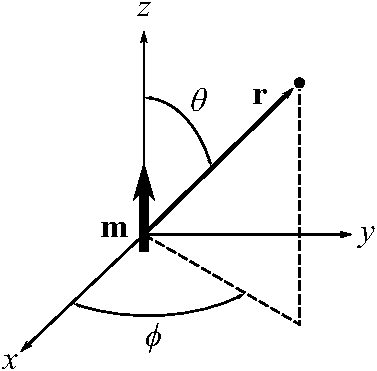
\includegraphics[width=4cm]{ch2/img/coord_pol_cart.pdf}
	\tdplotsetmaincoords{70}{110}
	\begin{tikzpicture}[auto,>=latex,tdplot_main_coords]
		\coordinate (origin) at (0,0,0);
		\tdplotsetrotatedcoords{-45}{-90}{0}
		\tdplotsetrotatedcoordsorigin{(origin)}
		%\riferimento
		% Axis
		\draw [->] (origin) -- (3,0,0) node[anchor=north east]{\scriptsize{$x$}}; \draw (origin) -- (-0.2,0,0);
		\draw [->] (origin) -- (0,2.5,0) node[anchor=west]{\scriptsize{$y$}}; \draw (origin) -- (0,-0.2,0);
		\draw [->] (origin) -- (0,0,2.5) node[anchor=south]{\scriptsize{$z$}}; \draw (origin) -- (0,0,-0.2);

		\draw[->,line width=2] (0,0,-0.1) -- node[left]{$\hat{\mathbf{m}}$} (0,0,1.5);
		\node [circle,draw,inner sep=1pt, fill=black] at (3,3,3) (rpoint) {};
		\draw [->] (origin) -- node[pos=0.8,above]{$\mathbf{r}$} (rpoint);
		\draw [dashed] (origin) -- (3,3,0) -- (3,3,3);
		\draw[tdplot_rotated_coords,<->] (2,0) arc (0:55:2) node[pos=0.5]{$\theta$};
		\draw [<->] (2,0,0) arc (0:45:2) node[pos=0.5,below]{$\phi$};
	\end{tikzpicture}
	\caption{From Polar coordinates to Cartesian coordinates}
	\label{fig:polar2cartesian}
\end{marginfigure}
\begin{marginfigure}
	\centering
	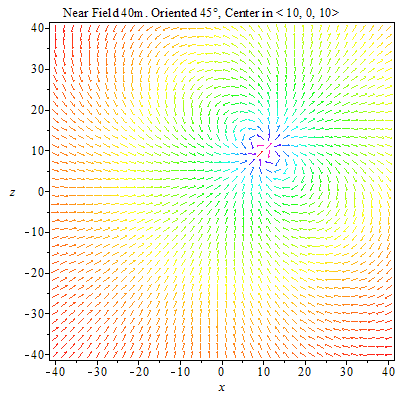
\includegraphics[width=5cm]{ch2/img/campo_casuale.png}
	\caption{Representation of a magnetic field with source: \newline $\postx = [10, 0, 10]^T$ \newline $\magdipole=[\ccos{\pi/4},0,\ssin{\pi/4}]^T$}
	\label{fig:dipolomagneticocasuale}
\end{marginfigure}
The last approximation is related to the nature of the receiver:
\begin{itemize}
\item the receiver act as an identifier of the constant quantity of the field, or the magnitude of the oscillating field
\item the distance of the receiver is always in a radius that allows us to not consider the effect of retarded potential: 
		\[\tau = \left. t - \dfrac{r}{c} \;\right|_{r\ll c}  \longrightarrow t \]
\end{itemize}

Under those considerations, and with MacLaurin first order transformation of $B_{\theta}$, the formulation of magnetic field real part takes the form:
\begin{equation}
\bfield = \dfrac{\magperm_0}{4 \pi r^3} \braces{ 2 m_0 \ccos{\theta} \vers{r} + m_0 \ssin{\theta} \vrtheta }
\label{eq:magneticfieldpolar}
\end{equation}

The projection of the field in cartesian coordinates is:
\begin{equation}
\bfield(\radiodist,\magdipole) = \dfrac{\magperm_0}{4 \pi r^5} \magfieldmatrix \magdipole
\end{equation}
A final generalization grants us the ability to write a general form of the field that has origin in position different from the origin:
\begin{equation}
\bfield(\hexastate - \postx,\magdipole)
\end{equation}
That is the form used for our simulations.

\section{Analytical signal analysis - A1--A \label{sec:a1asegnale}}

The ARTVA signal is a wild-life tag, specifically an \textbf{A--1A} signal. From the normative\cite{NormativaARVA}:
\begin{itemize}
\item A1A Signal:
	\begin{itemize}
	\item amplitude modulated signal
	\item digital information (keying)
	\item carrier frequency: \num{457}\si{\kilo\hertz}
	\item no auxiliary carrier
	\item frequency error shall not exceed $\pm$\num{80}\si{\hertz}
	\end{itemize}
\item carrier keying characteristics:
	\begin{itemize}
	\item on-time: \num{70}\si{\milli\second} minimum
	\item off-time: \num{400}\si{\milli\second} minimum
	\item period: \num{1000}\si{\milli\second} $\pm$ \num{300}\si{\milli\second}
	\end{itemize}
\item H--field peak at \num{10}\si{\meter}
	\begin{itemize}
	\item must be greater than \num{0.5}\si{\micro\ampere\per\meter}
	\item must be lower than \num{2.23}\si{\micro\ampere\per\meter}
	\end{itemize}
\end{itemize}

\begin{marginfigure}
	\centering
	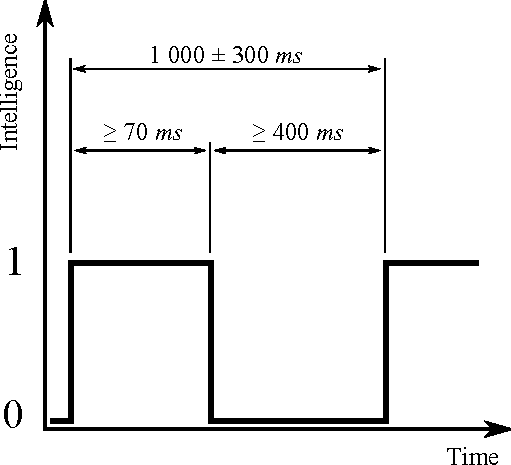
\includegraphics[width=5cm]{ch1/img/artva_signal.pdf}
	\caption{Intelligence signal of avalanche beacons}
	\label{fig:squarewaves}
\end{marginfigure}

The variable duty cycle is a challenge for the formulation of a searching algorithm, with a duty cycle ($\dutycycle$) that varies from a minimum of 5.4\% to a maximum of 42.9\%. The amplitude modulation, from a mathematical point of view is:
\begin{equation}
\jtx(t) = \braces{1+\mu \,\jint}\ccos{\omegaarva t}
\end{equation}
\begin{marginfigure}
	\centering
	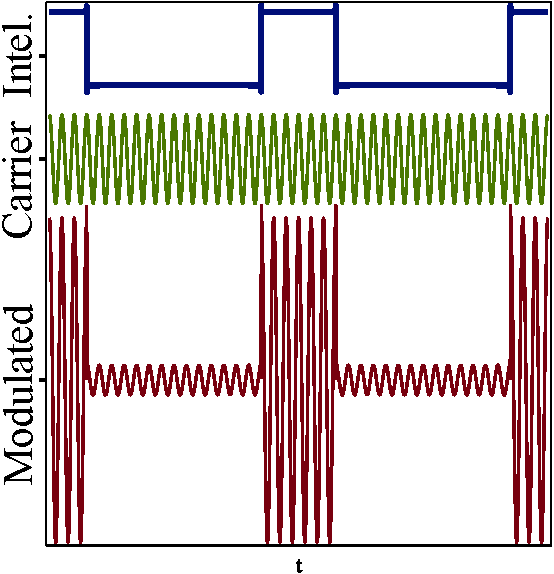
\includegraphics[width=5cm]{ch2/img/modulation_example.pdf}
	%\forceversofloat
	\caption{Example of a A--1A modulated signal}
	%\forceversofloat
\end{marginfigure}
There are 3 key elements:
\begin{itemize}
\item $\jint$ is the current of the intelligence signal, the representation of the square wave in figure \ref{fig:squarewaves}:
\begin{equation}
\jint(t) = A\dutycycle + \sum\limits_{n=1}^{\infty}\braces{\dfrac{2A}{n\pi}\ssin{n\pi \dutycycle} \ccos{\omegaint n t}}
\end{equation}
in which $A$ represents the signal amplitude and $\Delta$ is the duty cycle. 
\item the frequency of the carrier signal is ${f_0 = 2\pi\omegaarva}$, and it is \num{457}\si{\kilo\hertz}
\item $\mu$ is called modulation factor
\end{itemize}
From this current we are able to obtain the magnitude of dipole magnetic vector, using equation \ref{eq:dipolodacorrente}. Many of those parameter are device dependent and not known.

\section{Receiving antenna}

To receive such a long wavelenght for our appplication there is almost only one solution: use a ferrite core loop antenna, that is also the antenna used for transmission. In the next section, ferrite antenna is analyzed deeply, as a crucial part for the receiver. As we will see from the prototype, obtain a good receiver antenna is a very difficult task.

\subsection{Coils receiver}

\myparagraph{Single coil receiver}
\begin{marginfigure}
	\centering
	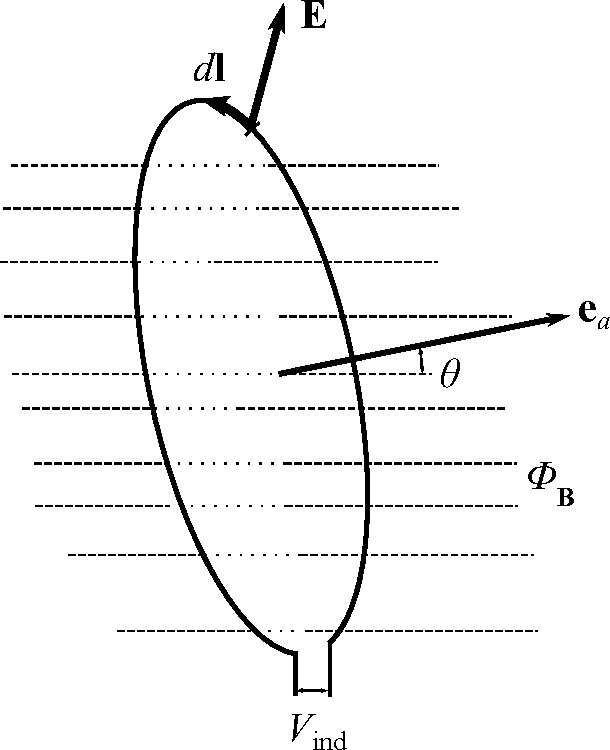
\includegraphics[width=5cm]{ch2/img/spira_singola.pdf}
	\caption{Single coil in field}
\end{marginfigure}
Under the hypothesys of an uniform EM field, using Maxwell's equations it is possible to derive potential difference induced in the coil:
\begin{equation}
\label{eq:tensioneindotta}
\vind = \oint\limits_{\diameter}\efield\cdot\mathbf{l} = -\dfrac{d\Phi_{\bfield}}{dt}
\end{equation}
where flux is:
\begin{equation}
\begin{array}{rcl}
\Phi_{\bfield} & = & \int\limits_{A_c} \bfield \cdot \hat{\mathbf{e}}_a dA \\
 & = & \magperm_0 H A \ccos{\theta}
\end{array}
\end{equation}
It is evident a cosine relation between field and axiis of the coil. The value of induced potential is maximum when the magnetic field $\hfield$ is orthogonal to the coil. $\theta$ is the angle between the field an the axis of the coil. Fusing two previous equations, we get:
\[
\vind = \magperm_0 A_c \dfrac{dH}{dt}
\]
that for our example:
\[
\vind = -j \omegaarva H A_c \magperm_0
\]
For conformity with the litterature, we express the magnetic field in terms of electric field\sidenote{It is known that: \newline $\magperm_{0} H = \dfrac{E}{\velocitaluce}$}:
\begin{equation}
\vind = \omegaarva \numerospire A_c \dfrac{E}{\velocitaluce}
\end{equation}

\myparagraph{Ferrite effect}
Inserting a ferrite bar brings to a deviation of the magnetic field flux. Fields lines are bended inside the ferrite because of its grater magnetic permeability
\begin{figure}
	\centering
	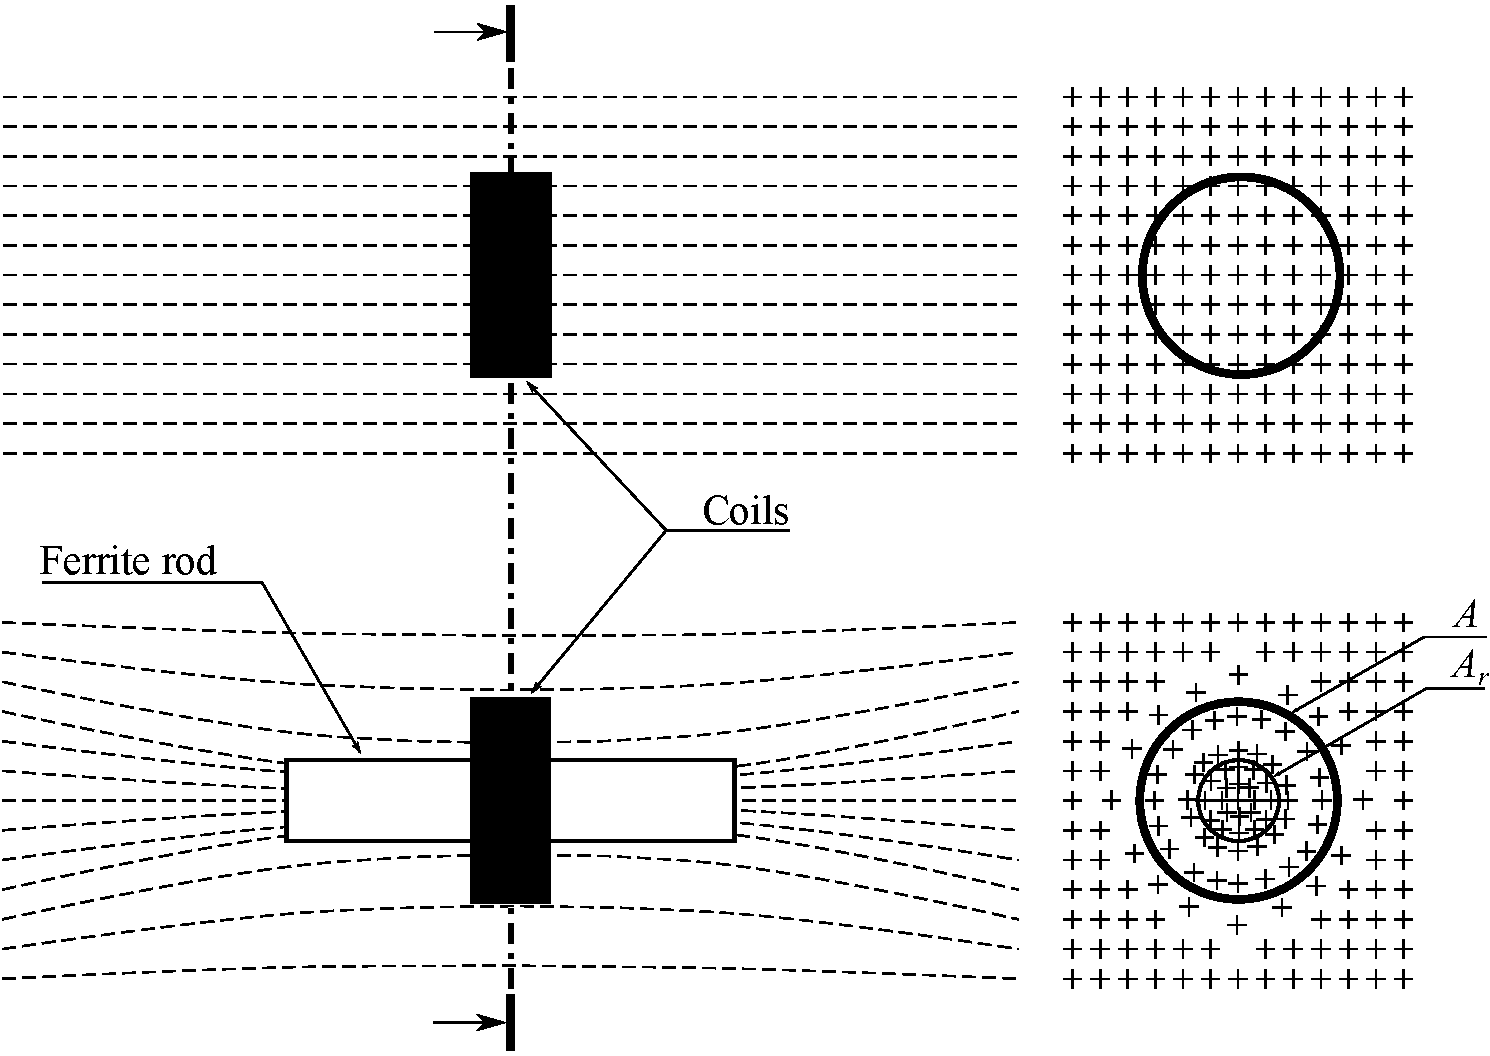
\includegraphics[width=11cm]{ch2/img/flux_lines.pdf}
	\label{fig:flussoferrite}
	\caption{Flux lines through coil and ferrite rod}
	\forceversofloat
\end{figure}
The total flux in section $A$ of figure \ref{fig:flussoferrite} is given by the flux that crosses area $A-A_r$ and flux that crosses area $A_r$:
\arraymath{
	\Phi_T & = & \Phi_{\bfield_1} + \Phi_{\bfield_2} \\
	\Phi_{\bfield_1} & = & \magperm_r A_r H \\
	\Phi_{\bfield_2} & = &\magperm_0 (A-A_r) H
}
and thus the total field is:
\begin{equation}
\Phi_T = H A_r \braces{ \magperm_r + \magperm_0 \braces{ \dfrac{A}{A_r} - 1} }
\end{equation}
bringing the previous equation in \ref{eq:tensioneindotta}, and simplifying with respect to constant parts of area, we get:
\begin{equation}
\vind = \omegaarva \numerospire \dfrac{E}{c} A_r \braces{\magperm_r + \braces{\dfrac{\diameter_c^2}{\diameter_r^2}-1}}
\end{equation}
In a real coil, we have a coil diameter that is equal to $\diameter_c = \diameter_c' + \diameter_\mathrm{wire}$, and it is usual to approximate $\diameter_c \approx \diameter_r$, and our antenna equation becomes:
\begin{equation}
\vind = \omegaarva \numerospire \dfrac{E}{c} A_r \magperm_r
\end{equation}
From which appears that the insertion of a ferrite rod in a coils inductance brings to an increase of induced tension proportional to the value of magnetic permeability of the ferrite itself. The identification of this value is not trivial and should be done experimentally. There are only some numerical approximation to the value of $\magperm_0$ related to the dimensions of ferrite bar, but it appears evidently a correlation between the ratio bar length/bar diameter. The greater this ratio, the greater the value of permeability\sidenote{We could give a trivial interpretation of this statement: the greater the length of the ferrite bar, the greater the number of flux lines that are bended into the bar; also the smaller the diameter, the grater the density of bended flux lines, thus the greater permeability value.}. 
\begin{equation}
\magperm_r \propto \dfrac{l_r}{\diameter_r}
\end{equation}

\myparagraph{Antenna effective height}
Effective height of antenna is defined as the ratio between the induced potential in the coils end the electric field intensity:
\begin{equation}
\altezzaeffettiva = \dfrac{\vind}{E}
\end{equation}
Applying previous equation to the definition of effective height:
\begin{equation}
\altezzaeffettiva = \dfrac{\omegaarva \numerospire A_r}{c} \braces{\magperm_r + \braces{\dfrac{\diameter_c^2}{\diameter_r^2}-1}}
\end{equation}

\subsection{Equivalent circuit and noise}
From a pure circuit point of view, ferrite antenna is seen as an an RLC circuit, in which we identify three passive components:
\begin{itemize}
\item $L\rightarrow\mathbf{Z}_L = j\omega L$: coil inductance
\item $R_p\rightarrow\mathbf{Z}_R = R_p$: wire resistance
\item $C\rightarrow\mathbf{Z}_C = (j\omega L)^{-1}$: parassite capacitance
\end{itemize}
The input voltage of the circuit is $\vind=\altezzaeffettiva E$
\begin{marginfigure}
	\centering
	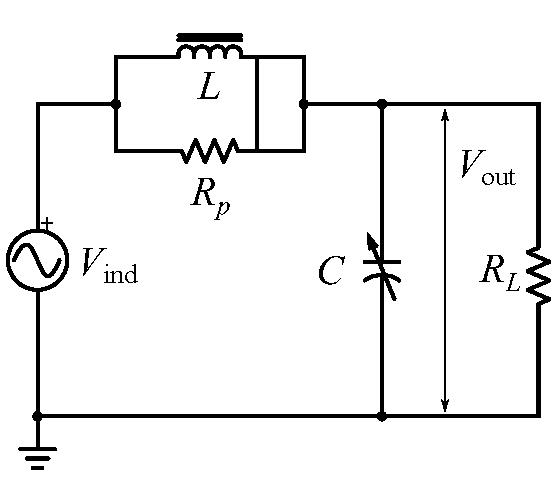
\includegraphics[width=5cm]{ch2/img/circuito_eq.pdf}
	\caption{Antenna equivalent circuit}
\end{marginfigure}

\myparagraph{Signal}
Starting from the definition of the equivalent circuit, with an external resistive load $R_L$ it is possible to derive a transfer function (full derivation in appendix at equation \ref{eq:transferfunc}):
\begin{equation}
\dfrac{V_{\mathrm{out}}}{\vind} = G(s) = \dfrac{\omega_{LC}}{Q_{\alpha}} \dfrac{s + Q_{\alpha} \omega_{LC}}{s^2 + \dfrac{\omega_{LC}}{Q_{\beta}} s + \omega_{LC}^2}
\end{equation}
\marginnote{\arraymath{
	\omega_{LC}^2 & = & \dfrac{1}{LC} \\
	Q_{\alpha} & = & \omega_{LC} R_P C \\
	Q_{\beta} & = & \omega_{LC} \dfrac{R_P R_L}{R_P + R_L} C
}}
if we obtain an $\omega_{LC} = \omegaarva$, we get resonance for an ARTVA incident signal: $s=j\omegaarva$:
\begin{equation}
G(j\omegaarva) = \left( -j Q_{\beta} \right) \left( 1 + \dfrac{j}{Q_{\alpha}} \right)
\end{equation} 
and then:
\begin{equation}
V_{\mathrm{out}} = \altezzaeffettiva \dfrac{Q_{\beta}}{Q_{\alpha}} E
\end{equation}

\myparagraph{Noise}
We could consider different sources of noise for our ferrite antenna:
\begin{itemize}
\item Boltzmann temperature noise
\item ferrite polarization noise
\item skin effect noise
\item auto-inductance noise
\end{itemize}

Even if some of those source are easily to model, some of them are not and require an experimental interpolation. For the Boltzmann withe noise:
\[
V_{n,B} = \sqrt{4 \boltzmann T \Delta f Q_{\beta} \mathbf{Z}_{L}}
\]
that is environment dependent. For the other sources, some more considerations must be driven. Skin effect and ferrite noise are proportional to the received field. 
Those two effects must be carefully taken into account and analyzed from experimental point of view. The first one is due to the distribution of the current in the section of the coil wire: current tends to accumulate in the skin layer of the wire, generating eddy currents that are sources of noise. To this effect, some special woven wire, like litz wire, should be used.
The second effect, ferrite noise, derives from the polarization of the magnetic crystal inside ferrite. To polarize the whole ferrite bar, some energy must be spent to move magnetic domain, and the movement of those domain generates a noise. This effect is strictly related to the quality of material and cannot be mitigated.
Auto-inductance noise is due to the current that is absorbed by the serial circuit of antenna and load. In a production of a prototype it is important that input of identification circuit has a very high impedance to reduce a generation of this current on antenna. Some high quality devices implement a secondary loop on the antenna that acts as a re-generator, that tries to null those parasitic currents effect.

It is straightforward now, that all those noise effect could be resumed in an unique interpolated expression $n \braces{\vind,T}$.

For simulation purpose it is possible to simulate this as Gaussian white noise as follows:
\begin{equation}
\sigma = N\braces{\mathbf{0}, V_{n,B}} + 10^{x} \abs{\vind} N\braces{\mathbf{0}, \Sigma}
\end{equation}
with $x$ a value that scales the proportional noise.
\section{Digital ARTVA prototype}
\begin{figure*}
	\centering
	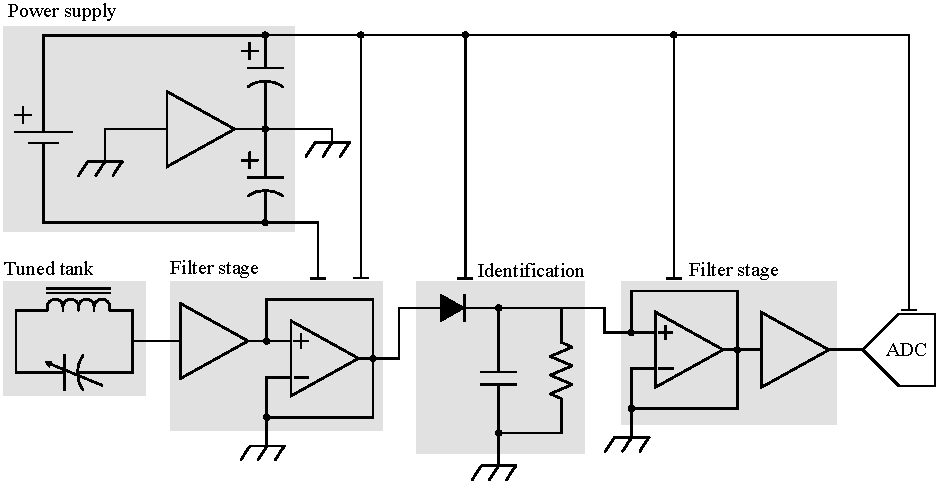
\includegraphics[scale=0.7]{ch2/img/block_circuit.pdf}
	\caption{Block diagram for the circuit}
	\label{fig:block_circuit}	
\end{figure*}
In the last section of this chapter, we use the knowledge collected to develop a prototype of an ARTVA receiver, in which there is not a transmission part. The receiver is the only fundamental module that we need for our drone, a transmitter will only be useless weight. 

In figure \ref{fig:block_circuit} there is the block outline of the device:
\begin{itemize}
\item the first block is the tuned tank, or tuned amplifier
\item the second block is the buffer and conditioner stage
\item the third block is the identification part
\item an amplification and a second buffer
\item digital component
\item dual supply stage
\end{itemize}
Through this section, each block will be discussed and explained. The design process has taken into account the tollerances for passive components\sidenote{Resistors: 5\%\newline Capacitors: 20\%}

\subsection{Tuned tank}
% \begin{figure}[b]
% 	\includegraphics[viewport=x y x y]{ch2/img/receiver3.pdf}
% 	\caption{}
% 	\label{fig:circuit}
% 	%\forceversofloat
% \end{figure}
\begin{figure}[h]
	\centering
	\includegraphics*[viewport=3 3 240 457,scale=0.4]{ch2/img/receiver3.pdf}
	\caption{Tuned tank portion of circuit}
	\label{fig:tunedtank}
	%\forceversofloat
\end{figure}

The tuned tank is composed by a ferrite antenna, with a rod of \num{10}\si{\centi\meter} per \diameter \num{1}\si{\centi\meter}. The wire of the coil is a \num{30} AWG enameled copper wire, with a final parasite resistance of \num{22}\si{\ohm}. The coil as \num{70} windings. For more informations about this tuned circuit, check previous section.

\subsection{Buffer and filter}
\begin{figure*}[h]
	\centering
	\includegraphics*[viewport=170 3 1250 380,scale=0.4]{ch2/img/receiver3.pdf}
	\caption{First filter stage}
	\label{fig:filter1}
	%\forceversofloat
\end{figure*}

This block is composed by a first stage that acts as a separation between the tuned tank and the filter, thus is also called voltage follower. To limit the number of components on the board this stage is obtained with an operational amplifier. To grant a longer receiving range, an high--gain selective active filter is in cascade to the buffer before the identification. It is important to select an operational amplifier with an high bandwidth--gain--product to grant the gain at \num{457}\si{\kilo\hertz}, at which the filter is centered. Also, this stage depends to the dual \num{\pm 5}\si{\volt} supply stage. 
\begin{marginfigure}
	\centering
	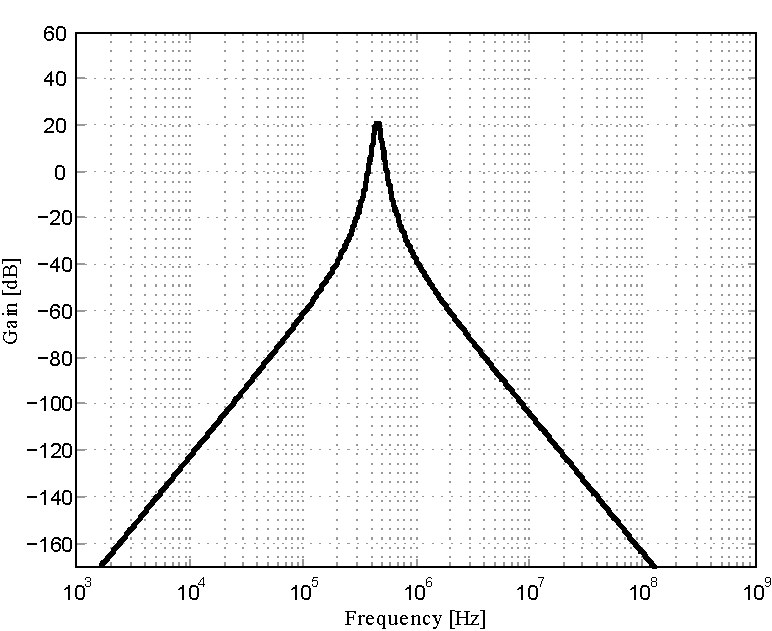
\includegraphics[width=5cm]{ch2/img/filter1.pdf}
	\caption{Filter magnitude characteristic}
\end{marginfigure}

The op--amp chosen is \texttt{LF347N}, even if a faster amplifier may be selected, it is advised to stay below the \num{60}\si{\mega\hertz} BW, to avoid auto--resonance effects.

\subsection{Identification}
\begin{figure}[h]
	\centering
	\includegraphics*[viewport=1251 3 1580 595,scale=0.4]{ch2/img/receiver3.pdf}
	\caption{Identification stage}
	\label{fig:identifier}
	%\forceversofloat
\end{figure}
\begin{marginfigure}
	\centering
	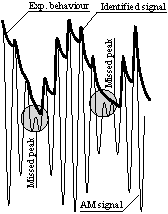
\includegraphics[width=4.5cm]{ch2/img/identificatore.pdf}
	\caption{Logical function of an identifier}
	\label{fig:identifier_log}
\end{marginfigure}
The central part of the circuit is an identification circuit, obtained with the monolithic classical IC \texttt{TA7641}\sidenote{A.k.a.: \texttt{MK484} or \texttt{ZN414}},  that acts as a one chip radio solution in AM. All receiver is derived from the modification of the basic circuit provided in schematics of this IC, extended with filtering and buffers, and the removal of the auto gain control resistance in the output feedback. Also, transistor amplification stage is removed. The output of this circuitry is in \numrange{40}{60}\si{\milli\volt}, with a very low current required. The input pin has a good impedance 

To better understand the use of this stage, look at figure \ref{fig:identifier_log}, in which an extremely simplified version of the IC is represented with common components. The IC straightens the received signal and identifies the envelope of the modulated intelligence with a low pass filter that has a dynamic not too slow, to not loose some of the higher frequencies information modulated (also called missed peak). IC implements this function with an high quality envelope detector.
\begin{figure*}[h]
	\centering
	\includegraphics*[viewport=1443 3 2320 350,scale=0.4]{ch2/img/receiver3.pdf}
	\caption{Low pass filter and amplification stage}
	\label{fig:filter2}
	\forceversofloat
\end{figure*}

\subsection{Amplifier}

The identified signal is, again, amplified and filtered, to a lower frequency, to grant the isolation of the square wave, with respect to the residual carrier and other source of interference. A \num{10}\si{\decibel} gain filter, with 2 stages was implemented. After the filter, another buffer connects analog circuitry with digital micro--controller.
\begin{marginfigure}
	\centering
	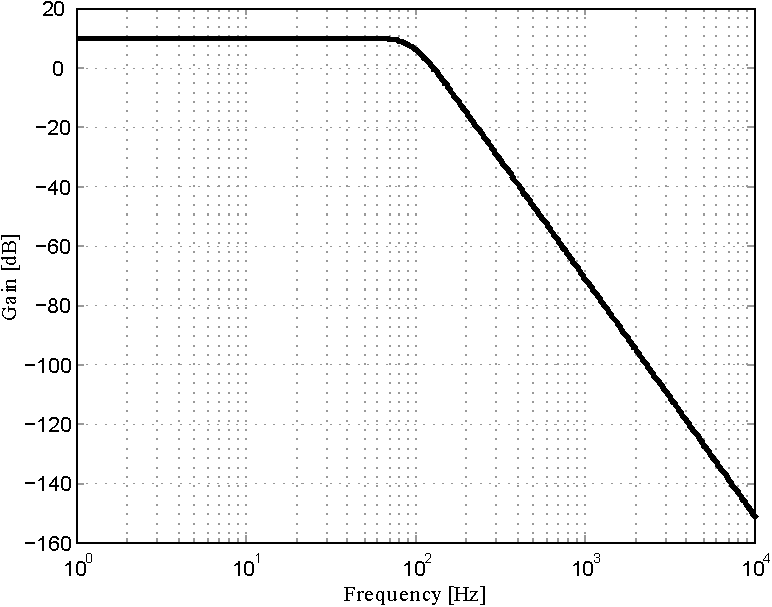
\includegraphics[width=5cm]{ch2/img/filter2.pdf}
	\caption{Filter magnitude characteristic}
\end{marginfigure}

\subsection{Digital stage}
\begin{figure}[h]
	\centering
	\includegraphics*[viewport=2320 3 2650 350,scale=0.4]{ch2/img/receiver3.pdf}
	\caption{Digital stage}
	\label{fig:adc}
	%\forceversofloat
\end{figure}
One last stage is he ADC and the UART interface on the micro--controller. Using an \texttt{MSP430} it is easy to develop in \texttt{C} the routines necessary to perform the task. To reduce the power consumption, ADC sampling is performed with ALU in power saving mode. Once the sampling task is completed, an interrupt brings up the ALU that set up the variables too be sent over serial interface UART (or SPI or I2C).

\subsection{Dual supply}
The supply is obtained through the use of a virtual ground and a symmetrical classical regulation circuit. This scheme is sometimes called rail splitter, and it is necessary for the first regulation stage, to avoid op--amps saturation.
\begin{figure}[h]
	\centering
	\includegraphics*[viewport=3 450 580 750,scale=0.4]{ch2/img/receiver3.pdf}
	\caption{Example of a sampling result}
	\label{fig:sampling_res}
	\forceversofloat
\end{figure}

\subsection{Tri--axes ARTVA}
In figure \ref{fig:sampling_res} there is an example of sampling from the real prototype, using MATLAB serial reading capabilities. A complete prototype uses three equal antenna--filter--identification--amplifier stage, with orthogonal antennas, and one single ADC micro--controller and power supply.
\begin{figure}[h]
	\centering
	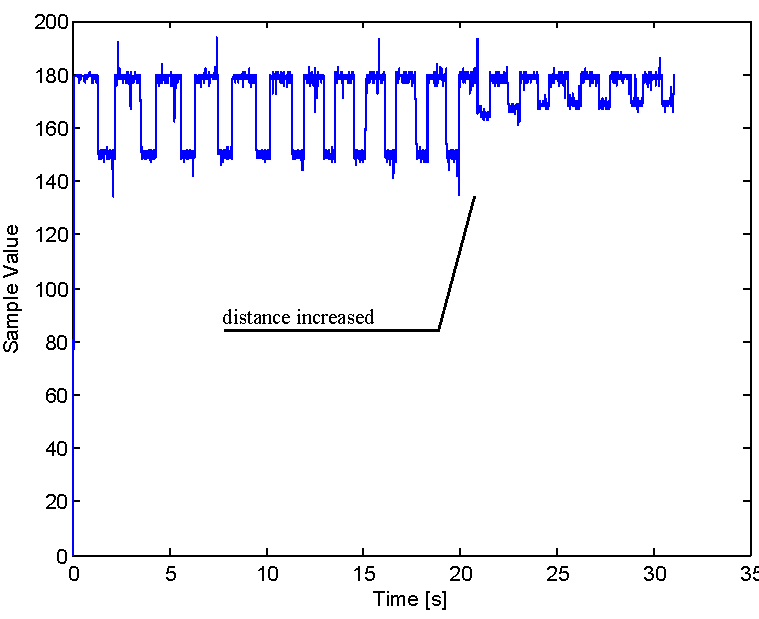
\includegraphics[scale=0.65]{ch2/img/sampling_result.pdf}
	\caption{Complete circuit}
	\label{fig:completecirc}
	%\forceversofloat
\end{figure}
\begin{figure}[p]
	\centering
	\includegraphics[scale=0.25,angle=90]{ch2/img/receiver3.pdf}
	\caption{Complete circuit}
	\label{fig:completecirc}
	\forceversofloat
\end{figure}

%\FloatBarrier
\clearpage
%%%%%%%%%% Appendix %%%%%%%%%%%%%%%%%%%%%%%%%%%%%%%%%%%%
% Appendix of chapter 2

\section{Appendix}

\subsection{Polar coordinates}

Maps:
\begin{equation} \left\{ \begin{array}{rcl} x & = & r \sin(\theta) \cos(\phi) \\ y & = & r \sin(\theta) \sin(\phi) \\ z & = & r \cos(\theta) \end{array}\right. \rightarrow \left\{ \begin{array}{rcl} r & = & \sqrt{x^2+y^2+z^2} \\ \theta & = & \arctan\left(\dfrac{z}{\sqrt{x^2+y^2}}\right) \\ \phi & = & \arctan\left( \dfrac{x}{y} \right) \end{array} \right. \end{equation}

Versors in Cartesian coordinates:
\begin{equation} \left[ \begin{array}{ccc} \vrr & \vrtheta & \vrphi \end{array}\right] = \dfrac{1}{\sqrt{x^2+y^2+z^2}} \left[ \begin{array}{ccc} x & \dfrac{xz}{\sqrt{x^2+y^2}} & -\dfrac{y}{\sqrt{x^2+y^2}} \\ y & -\dfrac{yz}{\sqrt{x^2+y^2}} & \dfrac{x}{\sqrt{x^2+y^2}} \\ z & -\dfrac{x^2+y^2}{\sqrt{x^2+y^2}} & 0 \end{array} \right] \end{equation}

\subsection{Evidences}

\myparagraph{EM field dynamic potential}
The following equations are the proof for \ref{eq:potvecmaxwell}
\begin{equation}
\begin{array}{rcl}
\nabla \cdot \left(  - \nabla \scpot - \partialtarg{\afield} \right) & = & \dfrac{\chargedens}{\dielettrico_0} \\
\nabla^2 \scpot + \partialt{\nabla \cdot \afield} & = & -\dfrac{\chargedens}{\dielettrico_0} \\
 & & \\
\magperm_0 \left( \currdens + \dielettrico_0 \partialt\left(- \nabla \scpot - \partialtarg{\afield}\right) \right) & = & \nabla \times \left( \nabla \times \afield \right) \\
\magperm_0 \currdens - \magperm_0 \dielettrico_0 \dfrac{\partial^2 \afield}{\partial t^2} - \magperm_0 \dielettrico_0 \nabla \dfrac{\partial \scpot}{\partial t} & = & \nabla \left( \nabla \cdot \afield \right) - \nabla^2 \afield \\
\nabla^2 \afield - \dfrac{1}{c^2} \dfrac{\partial^2 \afield}{\partial t^2} - \nabla \left( \nabla \cdot \afield + \dfrac{1}{c^2} \dfrac{\partial \scpot}{\partial t} \right) & = & - \magperm_0 \currdens
\end{array}
\label{eq:evidence1}
\end{equation}

In the following equation invariance with respect to recalibration map is showed:
\begin{equation}
\label{eq:prooftransformationmap}
\begin{array}{rcl}
\nabla \times \afield' & = & \nabla(\afield + \nabla \lorentz) \\
 & = & \nabla \times \afield + \nabla \times \nabla \lorentz \\
 & = & \nabla \times \afield \\
 & = & \bfield \\
 & & \\
- \nabla\scpot' - \partialtarg{\afield'} & = & -\nabla \left( \scpot - \partialtarg{\lorentz} \right) - \partialt\left( \afield + \nabla \lorentz \right) \\
 & = & -\nabla \scpot + \nabla \partialt \lorentz - \partialtarg{\afield} - \partialt\nabla\lorentz \\
 & = & -\nabla \scpot - \partialtarg{\afield} \\
 & = & \efield
\end{array}
\end{equation}

\myparagraph{Magnetic dipole radiation}
To evaluate the integral \ref{eq:integraledacalc}  we should consider some simplifications.

$r' \ll r$: for an ideal dipole, coils radius shall be really with respect to radio vector:
\[
\begin{array}{rcl}
\kappa & = & \sqrt{(\radiodist - \radiodist') \cdot (\radiodist - \radiodist')} = \\
 & = & \sqrt{\radiodist \cdot \radiodist + \radiodist' \cdot \radiodist' - 2\; \radiodist \cdot \radiodist'} \\
 & = & \sqrt{r^2 + r'^2 - 2\,r\,r'\,sin(\theta)cos(\varphi')} \\
 & = & r\;\sqrt{1 + \dfrac{r'^2}{r^2} - 2\,\dfrac{r'}{r}\,sin(\theta)cos(\varphi')}
\end{array}
\]
the simplification is performed by the use of Taylor expansions, under the hypothesis of $r'^2/r^2 \approx 0$:
\arraymath{
\kappa & = & \mathrm{Taylor}_2\left[ r\;\sqrt{1 - 2\,\dfrac{r'}{r}\,sin(\theta)cos(\varphi')} \right]_{\dfrac{r'}{r} \rightarrow 0} \\
 & \approx & r\left( 1 - \dfrac{r'}{r}\,sin(\theta)cos(\varphi') \right)
}
imposing the inverse:
\arraymath{
\dfrac{1}{\kappa} & = & \dfrac{1}{r}\left( 1 - \dfrac{r'}{r}\,sin(\theta)cos(\varphi') \right)^{-1} \\
 & = & \mathrm{Taylor}_2\left[ \dfrac{1}{r}\left( 1 - \dfrac{r'}{r}\,sin(\theta)cos(\varphi') \right)^{-1} \right]_{\dfrac{r'}{r} \rightarrow 0} \\
 & \approx & \dfrac{1}{r}\left( 1 - \dfrac{r'}{r}\,sin(\theta)cos(\varphi') \right)
}

$r' \ll \lambda = 2\pi\velocitaluce/\omegaarva$: this observation permits us to simplify the cosine in the argument of the integral, with $\tau$ as defined in \ref{eq:campidef1}:
\marginnote{$\cos(\gamma + \beta) = \cos\gamma\cos\beta - \sin\gamma\sin\beta$\\for $\gamma\rightarrow0$ we get $\ssin{\gamma} \approx \omegaarva\tau$ and $\ccos{\gamma} \approx 1$}
\arraymath{
\ccos{\omegaarva \left( t - \dfrac{\kappa}{\velocitaluce}\right)} & \approx & \ccos{\omegaarva\tau} + \dfrac{\omegaarva r'}{\velocitaluce} \ssin{\theta} \ccos{\varphi'} \\
 & = & \ccos{\omegaarva\tau}\ccos{\dfrac{\omegaarva r'}{\velocitaluce} \ssin{\theta} \ccos{\varphi'}} - \\
 &   & + \ssin{\omegaarva\tau} \ssin{\dfrac{\omegaarva r'}{\velocitaluce} \ssin{\theta} \ccos{\varphi'}} \\
 & \approx & \ccos{\omegaarva\tau} - \\ & & + \ssin{\omegaarva\tau} \ssin{\dfrac{\omegaarva r'}{\velocitaluce} \ssin{\theta} \ccos{\varphi'}}
}

The union of the two simplifications give us as integral argument:
\[\begin{array}{l}
\dfrac{1}{r}\braces{1+\dfrac{r' \ccos{\theta} \ssin{\varphi'}}{r}} \cdot \\
\cdot \braces{\ccos{\omegaarva\tau} - \dfrac{\omegaarva r' \ssin{\theta} \ccos{\varphi'}\ssin{\omegaarva\tau}}{\velocitaluce}}
\end{array}\]
expanding and considering $\xi = \ssin{\theta}\ccos{\varphi'}$ we obtain:
\[
\dfrac{1}{r} \braces{ \dfrac{\omegaarva\ssin{\omegaarva\tau}\xi r'}{c} + \ccos{\omegaarva\tau} - \dfrac{\omegaarva\ssin{\omegaarva\tau}\xi r'^2}{cr} + \dfrac{\ccos{\omegaarva\tau}\xi r'}{r} }
\]
where the term $\frac{r'^2}{cr} = \frac{r'}{r}\;\frac{\omegaarva}{2\pi}\;\frac{r'}{\lambda} \approx 0$ as we have already stated:
\[
\dfrac{1}{r} \braces{ \ccos{\omegaarva\tau} -\braces{\dfrac{\omegaarva}{c}\ssin{\omegaarva\tau} - \dfrac{1}{r}\ccos{\omegaarva\tau}}r'\xi}
\]
extracting only the parts that are function of integration variable $\varphi'$:
\arraymath{
a_1 & = & \dfrac{1}{r} \ccos{\omegaarva\tau} \\
a_2 & = & \dfrac{1}{r} \braces{\dfrac{\omegaarva}{c}\ssin{\omegaarva\tau} - \dfrac{1}{r}\ccos{\omegaarva\tau}}r'\ssin{\theta}
}
The final integral is in the form:
\[
\afield(\radiodist,t) = \dfrac{\magperm_0 J_0 r'}{4\pi r} \int\limits_{0}^{2\pi}a_1 \ccos{\varphi'} - a_2 \cos^2\braces{\varphi'} d\varphi' \hat{\phi}
\]
and thus solved:
\marginnote{$\begin{array}{l} \int\limits_0^{2\pi}\ccos{\varphi'}d\varphi' = 0 \\ \int\limits_0^{2\pi}\cos^2\braces{\varphi'}d\varphi' = \pi \end{array}$}
\arraymath{
\afield(\radiodist,t) & = & -\dfrac{\magperm_0 J_0 r'}{4\pi} \pi a_2 \\
 & = & \dfrac{\magperm_0 J_0 r'^2 \pi}{4\pi r} \braces{\dfrac{1}{r}\ccos{\omegaarva\tau} - \dfrac{\omegaarva}{c}\ssin{\omegaarva\tau}}
}
Applying the substitution $m_0 = \pi r'^2 J_0$ we found the solution reported in equation \ref{eq:soluzioneint}.

\myparagraph{Complex version of magnetic field}
Here the proof of complex magnetic field equations:
\[
\begin{array}{rcl}
B_r & = & \dfrac{1}{2} \dfrac{\magperm_0 m_0}{\pi} \ccos{\theta} \braces{\dfrac{1}{r^3}\ccos{\omegaarva \tau} - \dfrac{\kappa}{r^2} \ssin{\omegaarva \tau}} \\
 & = & \dfrac{1}{2} \dfrac{\magperm_0 m_0}{\pi} \ccos{\theta} \kappa^3 \braces{ \dfrac{1}{r^3 \kappa^3} \ccos{\omegaarva\tau} - \dfrac{1}{r^2 \kappa^2} \ssin{\omegaarva\tau} } \\
 & = & \dfrac{1}{2} \dfrac{\magperm_0 m_0}{\pi} \ccos{\theta} \kappa^3 \braces{ \dfrac{1}{r^3 \kappa^3} + \dfrac{j}{r^2 \kappa^2}} e^{j\omegaarva \tau} \\
 & = & \dfrac{1}{2} \dfrac{\magperm_0 m_0}{\pi} \ccos{\theta} \kappa^3 \braces{ \dfrac{j}{r^2 \kappa^2} + \dfrac{1}{r^3 \kappa^3}} e^{j\omegaarva \tau} \\
 & = & -\dfrac{1}{2} j \dfrac{\magperm_0 m_0}{\pi} \kappa^3 \ccos{\theta} \braces{\dfrac{1}{j^2 r^2 \kappa^2} + \dfrac{1}{j^3 r^3 \kappa^3}} e^{j\omegaarva \tau}
\end{array}
\]

\[
\begin{array}{rcl}
B_{\theta} & = & \dfrac{1}{4} \dfrac{\magperm_0 m_0}{\pi r^3 c^2} \ssin{\theta} \braces{\braces{\velocitaluce^2 - \omegaarva^2 r^2}\ccos{\omegaarva \tau} - \omegaarva r \velocitaluce \ssin{\omegaarva \tau}} \\
 & = & \dfrac{1}{4} \dfrac{\magperm_0 m_0}{\pi} \ssin{\theta} \braces{ \braces{\dfrac{1}{r^3}-\dfrac{\omegaarva^2}{c^2 r}}\ccos{\omegaarva \tau} - \dfrac{\omegaarva}{r^2 c} \ssin{\omegaarva \tau}} \\
 & = & \dfrac{1}{4} \dfrac{\magperm_0 m_0}{\pi} \ssin{\theta} \braces{ \braces{\dfrac{1}{r^3}-\dfrac{\kappa^2}{r}}\ccos{\omegaarva \tau} - \dfrac{\kappa}{r^2} \ssin{\omegaarva \tau}} \\
 & = & \dfrac{1}{4} \dfrac{\magperm_0 m_0}{\pi} \ssin{\theta} \kappa^3 \braces{ \braces{\dfrac{1}{r^3 \kappa^3}-\dfrac{1}{r \kappa}}\ccos{\omegaarva \tau} - \dfrac{1}{r^2 \kappa^2} \ssin{\omegaarva \tau}} \\
 & = & \dfrac{1}{4} \dfrac{\magperm_0 m_0}{\pi} \ssin{\theta} \kappa^3 \braces{ \braces{\dfrac{1}{r^3 \kappa^3}-\dfrac{1}{r \kappa}} + \dfrac{j}{r^2 \kappa^2}} e^{j\omegaarva \tau} \\
 & = & \dfrac{1}{4} \dfrac{\magperm_0 m_0}{\pi} \ssin{\theta} \kappa^3 \braces{-\dfrac{1}{r \kappa} + \dfrac{j}{r^2 \kappa^2} + \dfrac{1}{r^3 \kappa^3}} e^{j\omegaarva \tau} \\
 & = & -\dfrac{1}{4} j \dfrac{\magperm_0 m_0}{\pi} \kappa^3 \ssin{\theta} \braces{\dfrac{1}{j r \kappa} + \dfrac{1}{j^2 r^2 \kappa^2} + \dfrac{1}{j^3 r^3 \kappa^3}} e^{j\omegaarva \tau}
\end{array}
\]

\myparagraph{The field in cartesian coordinates}
From the figure \ref{fig:polar2cartesian} we derive the following relations:
\arraymath{
\vers{r} & = & \dfrac{\radiodist}{\abs{\radiodist}} \\
\vrtheta & = & \dfrac{ (\magdipole \times \radiodist) \times \radiodist }{ \abs{ (\magdipole \times \radiodist) \times \radiodist } } 
}
and the magnetic dipole vector is the projection on the two versors:
\arraymath{
\magdipole \cdot \vers{r} & = & m_0 \ccos{\theta}\\
\magdipole \cdot \vrtheta & = & -m_0 \ssin{\theta}
}
thus equation \ref{eq:magneticfieldpolar} becomes:
\arraymath{
\bfield & = & \dfrac{\magperm_0}{4 \pi r^3} \braces{ 2 m_0 \ccos{\theta} \vers{r} + m_0 \ssin{\theta} \vrtheta } \\
 & = & \dfrac{\magperm_0}{4 \pi r^3}\braces{2\braces{\magdipole \cdot \vers{r}} \vers{r} - \braces{\magdipole \cdot \vrtheta} \vartheta} \\ 
 & = & \dfrac{\magperm_0}{4 \pi r^3}\braces{3\braces{\magdipole \cdot \vers{r}} \vers{r} - \braces{\magdipole \cdot \vers{r}} \vers{r} - \braces{\magdipole \cdot \vrtheta} \vartheta} \\ 
 & = & \dfrac{\magperm_0}{4 \pi r^3}\braces{3\braces{\magdipole \cdot \vers{r}} \vers{r} - \magdipole}
}
putting the last equation in an analytical math engine, we derive this compact version, using as notation $\radiodist = [x,\,y,\,z]^T$:
\begin{equation}
\bfield = \dfrac{\magperm_0}{4 \pi r^5} \magfieldmatrix \magdipole
\end{equation}

\subsection{Antenna transfer function}
It is easy to derive transfer function, if we consider the system as a voltage divider:
\begin{equation}\label{eq:transferfunc}
\begin{array}{ccl}
\dfrac{V_{\mathrm{out}}}{\vind} & = & \dfrac{\left(R_L \parallel C s \right)}{\left(R_L \parallel C s \right) + \left(R_P \parallel L s \right)} \\
& = & \dfrac{\dfrac{1}{\dfrac{1}{R_L} + Cs}}{\dfrac{1}{\dfrac{1}{R_L} + Cs} + \dfrac{1}{\dfrac{1}{R_L} + \dfrac{1}{L s}}} \\
& = & \dfrac{ \dfrac{1}{R_p}+\dfrac{1}{Ls} }{ \dfrac{1}{R_L} + Cs + \dfrac{1}{R_P} + \dfrac{1}{Ls} } \\
& = & \dfrac{1}{R_P C} \dfrac{s + \dfrac{R_P}{L}}{s^2 + \dfrac{1}{C \dfrac{R_P R_L}{R_P + R_L}}s + \dfrac{1}{LC}} 
\end{array}
\end{equation}


